
\chapter*{Preface --- A personal, historical and audiophile
  dissertation}
\addcontentsline{toc}{chapter}{Preface --- A personal, historical and
  audiophile dissertation}

\begin{todo}{Juan Pedro}
  En el resto del doclumento uso el plural de modestia, pero aquí
  hablo en un tono más informal y en primera persona. La idea es
  introducir al lector, que probablemente esté totalmente
  desfamiliarizado con el tema, haciendo un recorrido cronológico en
  paralelo de la concepción y desarrollo del Psychosynth así como de
  mi interés por la música electrónica y de la música electrónica en
  sí (al fin y al cabo, mi interés por la música electrónica está
  ordenado por la su cronología también.). 

  Al final lo he pasado al prefacio. Si alguien cree mejor ponerlo en
  la introducción, pues que lo diga.
\end{todo}

I am going to let the formalities, both in form and content, of a
final project aside in this section to give an initial background on
the historical development of the conception of GNU Psychosynth. After
all, the story of this project is, in many ways, the story of my own
learning and maturing process and specially the evolution of my
interest in music.

In 2006 I was a young computer science student who had just moved to
Granada, a city full of youth, joy and cultural activities. At that
time, I was not keen at all in electronic music ---maybe biased by my
prejudices on the rave subculture that surrounds a wide part of it,
even though eventually I happened to appreciate it in some way. At
that time I was more of a punk and ska fan and rejected the
artificiality and production process of electronic music; this was
actually a contradiction with my interest in programming. However, I
eventually got specially interested in the wild 70's explosion of
musical experimentation, and concretely in progressive rock.

I can vividly remember my first positive contact with electronic
music. It was a chilled and psychedelic evening at a friend's place
---one of those old and rundown but magical flat, with rather high
ceilings and wooden windows, where many students live in Granada---
when we Youtubed a video where Keith Emerson virtuously performed
``Knife Edge'' on a keyboard attached to a big wooden box full of
wires and knobs. By rearranging the wires or playing with the knobs,
he would radically change the sound that his keyboard
emitted. That magical sound machine was a Moog modular synthesiser,
and that was the birth of a true love for electronic music that would
later conceive Psychosynth ---is not love, they say, the true means
for conception?

\begin{figure}[h!]
  \centering
  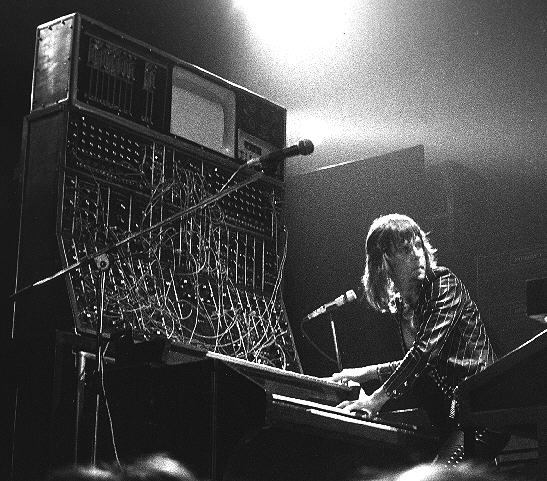
\includegraphics[width=.7\textwidth]{pic/elpmoog.jpg}
  \caption[Keith Emerson playing a modular Moog]{Keith Emerson playing
    a modular Moog. The keyboard is connected to a big rack of
    modules, interconnected with eachother with wires. Each module
    generates or processes the sound carried in analog form in the
    interconnecting wires, therefore having an exponential number of
    possibly different sounds by combining modules and settings.}
\end{figure}

After that, I started to listen to more and more music made with
electronic devices --- an exploration that happened, actually,
following electronic music's own history. From the synthesiser-full
rock of Soft Machine, King Crimson or The Nice I opened my ears to the
purely synthetic orchestral compositions of Wendy Carlos, Vangelis or
the early Jean Michelle Jarre. Kraftwerk's own evolution from rock to
drum-pads, vocoders and synthesisers allowed me to open my ears to
more modern electronic music.

\begin{figure}[h!]
  \centering
  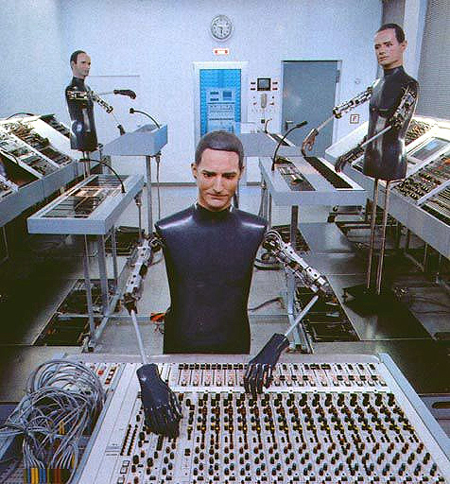
\includegraphics[width=.6\textwidth]{pic/kraftwerk.jpg}
  \caption[Artwork for the music of Kraftwerk]{Artwork for the music
    of Kraftwerk, with robotic representations of the band members
    playing with electronic instruments. On the front we can see an
    old analog sequencer. As opposed to a synthesizer ---this is, a
    virtual instrument, which is in charge of producing sound of
    whatever note you tell it to--- a \emph{sequencer} is an
    electronic score that can not produce sound by itself. The notes
    are programmed in the device ---in an analog sequencer, by
    toggling switches and knobs--- and it sends them at the
    appropriate time and duration to the electronic instruments
    (synthresisers) it is connected to. While current digital
    sequencers are very powerful, at that time they had important
    limitations that influenced Kraftwerk's robotic but charm
    sound. Kraftwerk was one of the first pop bands to produce its
    music entirely with electronic devices and is considered the
    father of modern electro and techno and has heavily influenced
    many other styles like house and hip-hop.}
\end{figure}

It was still my first year of university when I watched a video, under
circumstances probably similar to that before, of a new device being
developed in the University Pompeu Fabra, in Barcelona: the ReacTable
\cite{jorda07thereactable}. In a dark room only illuminated by a
bright blue table, several performers placed tagged objects on the
table. The table automatically arranged a connection graph among the
objects based on their nature and relative distance and it displayed
it but, more interestingly, the sound was evolving as this graph
did. I just thought: wow, that must be fun, I want to play with that!
--- well, Do It Yourself.

That was the birth of Psychosynth. At the beginning it was just a
toy. I did know nothing on how to process real-time audio, so I wrote
many experiments. When I was bored of testing the dynamic range of my
speakers and ears with all sorts of sinusoids, triangle and square
signals I started to read more and more source code of other audio
Free Software and eventually started to write a digital modular
synthesizer and play with Ogre3D. %\cite{ogre3d}.
\footnote{Torus Knot Software Ltd. \url{http://www.ogre3d.com}} By the
summer of 2007 I had some very primitive synthesis code and also some
user interface experiments\footnote{As this video can show,
  \url{http://blip.tv/file/325103}, the software was just a bunch of
  buttons with a 3D blue table like Reactable's and no sound.}. While
I was an average C developer when I started my studies, I did not have
any clue on C++. During the development of these initial experiments,
I also had to learn about inheritance, what \texttt{virtual} means,
etc. but of course the design was flawed all the time and I had to
rewrite the code many times.

\begin{figure}
  \centering
  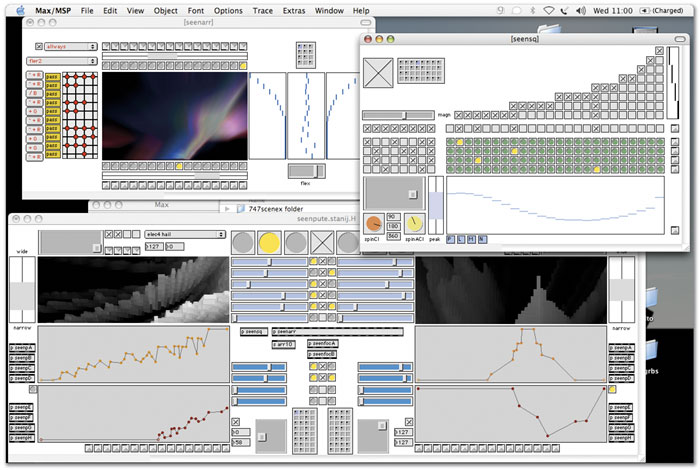
\includegraphics[width=.7\textwidth]{pic/autechre-2.jpg}
  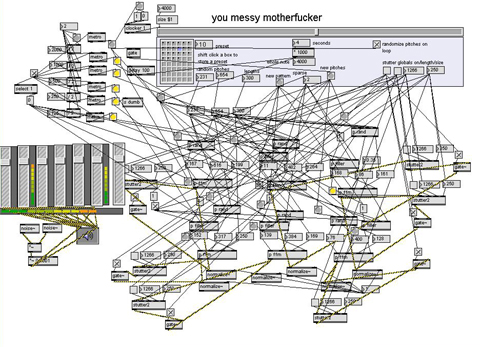
\includegraphics[width=.7\textwidth]{pic/autechre-1.jpg}
  \caption[Autechre related Max/MSP patches]{The first picture is a
    Max/MSP claimed to be made by the electronic music duo
    Autechre\cite{autechrepatch}. The second is a Max/MSP patch made
    by Robbie Martin that \emph{generatively} reverse-engineers Autechre's
    song Powmod. Music is said to be \emph{generative} when the whole
    composition itself is performed by pseudo-random algorithms
    programmed to produce well-sounding evolving non-repeating
    patterns. Autechre are known to have explored generative
    music. Max/MSP and its Free Software counterpart Pure Data are
    graphical data-flow programming software, which can be considered
    a low-level modular synthesizer, that is often used to write
    arbitrarily complex musical software and is specially interesting
    for generative music.}
  \label{fig:autechre}
\end{figure}

Something happened then at the beginning of my second year of
university: I applied as a contestant to the Spanish Free Software
Contest for University Students, and Psychosynth was the project I
would develop. At that time I was already interested in experimental
electronic music from the 90's, and late programming nights were
accompanied by Autechre's fractal glitchs and Aphex Twin and
Squarepusher's spastic patterns\footnote{If there is something I am
  grateful for during the early development of Psychosynth is the
  patience of my flatmates during those noisy programming
  nights. Psychosynth was long-time nicknamed ``the ambulance siren
  sound maker'' because it was only able to produce recursively
  modulated sinusoids.}. At that time, this cruise in the most
experimental side of electronic music and my ignorance in proper music
making made me believe in scoreless generative music produced from
evolving continuous signals, and that influenced the lack of proper
synchronisation mechanisms in Psychosynth. At some point,
Shaker08\footnote{\url{http://soundcloud.com/shaker08}}, a music producer
and DJ from Malaga, developed some beat loops to distribute along with
the software and helped in early showcase performances. He also
tough me a lot on how music is traditionally made.

The project won a price in that Free Software contest and he got some
reviews in blogs. it then became part of the GNU project --- an
attempt to assure its long-term development and that it would remain
Free Software in the future.

After that, however, the development stalled a bit. I had big
refactoring ideas that never got the motivation to be accomplished. In
that seek for perfect code motivated by an increasing interest in
programming language theory and functional and generic programming, I
also became more and more conscious of the flaws of the code
---i.e. the lack of synchronisation mechanisms, MIDI (Music Instrument
Digital Interface) support, pluggable modules, patch persistence,
etc.\ make any serious non-experimental attempt to make music with it
very hard. During these last 2 years I have learnt much more on the
music production workflow and terminology, a process parallel to a
final step in opening my ears to current electronic music, specially
Drum and Bass, Dubstep, and even some Minimal and Techno. During last
summer I got a MIDI DJ controller that got me to better understand the
limitations and possibilities of Psychosynth for music mixing and I
became a casual contributor of the best Free Software DJ software:
Mixxx \cite{andersen03mixxx}. Also, the people at
ArtQuimia\footnote{\url{http://www.artquimia.net/}}, the music production
school where Shaker08 was educated, became interested in the project
and has offered lending gear for testing and supervision, guidelines
and insight from a musician point of view.

So here we are now, in the fall of 2010. Still quite ignorant in music
making but pretending to be a ``digital luthier'' motivated by passion
for music. And trying to turn all this personal game into a final
master thesis project. Lets see how it goes\ldots


\begin{savequote}[10pc]
  \sffamily La utopía está en el horizonte. Camino dos pasos, ella se
  aleja dos pasos y el horizonte se corre diez pasos más
  allá. ¿Entonces para que sirve la utopía? Para eso, sirve para
  caminar.
  \qauthor{Eduardo Galeano}
\end{savequote}

\chapter{Introduction, definition and goals}

\section{Problem definition}

Our problem definition is well expressed in the title of this project:
``a framework for modular, interactive and collaborative sound
synthesis and live music performance''. Lets elaborate this by
describing its parts.

\subsection{A modular synthesiser}
\label{sec:defmodular}
A modular synthesiser is one where the sound generation and
manipulation process is described as a directional graph where each
link represents the flow of sound signal from one node to another, and
each node transforms or generates those signals.

A node with no input is often called a \emph{generator}. A node with
one input and one output is often called a \emph{filter}. A node can
have different \emph{parameters} that in analog hardware can be set
with knobs and potentiometers. Often, these parameter can be
controlled with other optional input signals that are called
\emph{modulators}. A concrete interconnection of a set of modules is
commonly referred as a \emph{patch}. Note \ref{note:modsynth} lists
some of the most common modules in analog modular synthesisers.

\begin{mynote}[Standard modules in an analog modular synthresizer]
  \label{note:modsynth} Software modular synthesizers have usually
  similar ones in their default module too, while they quite often use
  different terminology not related to this voltage based signal like
  in this case.
  
  \noindent [The following text is extracted from the Wikipedia
  article on ``Modular Synthesizer,'' as checked on December 12th
  2010.]
 
  \begin{description}
  \item[VCO] Voltage Controlled Oscillator, which will output a
    pitched sound (frequency) in a simple waveform (most usually a
    square wave or a sawtooth wave, but also includes pulse,
    triangle and sine waves).
  \item[Noise source] A generator that supplies ``hiss'' sound similar
    to static, which can be used for explosions, cymbals, or
    randomly generated control signals. Common types of noise
    offered by modular synthesizers include white, pink, and low
    frequency noise.
  \item[VCF] Voltage Controlled Filter, which attenuates frequencies
    below (high-pass), above (low-pass) or both below and above
    (band-pass) a certain frequency. VCFs can also be configured to
    provide band-exclusion, whereby the high and low frequencies
    remain while the middle frequencies are removed.
  \item[VCA] Voltage Controlled Amplifier, which varies the
    amplitude of a signal in response to a supplied control voltage.
  \item[EG] Triggering an Envelope Generator produces a single,
    repeatable shaped voltage pulse. Often configured as ADSR
    (Attack, Decay, Sustain, Release) it provides the means to shape
    a recognizable sound from a raw waveform. This technique can be
    used to synthesize the natural decay of a piano, or the sharp
    attack of a trumpet. It can be triggered by a keyboard or by
    another module in the system. Usually it drives the output of a
    VCA or VCF, but the patchable structure of the synthesizer makes
    it possible to use the envelope generator to modulate other
    parameters such as the pitch or pulse width of the VCO. Simpler
    EGs (AD or AR) or more complex (DADSR—Delay, Attack, Decay,
    Sustain, Release) are sometimes available.
  \item[LFO] A Low Frequency Oscillator is similar to a VCO but it
    usually operates below 20 Hz. It is generally used as a control
    voltage for another module. For example, modulating a VCO will
    create vibrato while modulating a VCA will create tremolo.
  \item[RM] Ring modulator, two audio inputs are utilized to create
    sum and difference frequencies while suppressing the original
    signals. This gives the sound a ``robotic'' quality.
  \item[Mixer] A module that combines multiple signals into one.
  \item[S\&H] Sample and hold, which takes a ``sample'' of the input
    voltage when a trigger pulse is received and ``holds'' it until a
    subsequent trigger pulse is applied. The source is often taken
    from a noise generator.  Sequencer, which produces a sequence of
    notes, usually a music loop.
  \item[Slew limiter] Smooths off the peaks of voltages. This can be
    used to create glide or portamento between notes. Can also work
    as a primitive low-pass filter.
  \item[Custom Control Inputs] Because modular synthesizers have
    voltage-driven inputs, it is possible to connect almost any kind
    of control. Pitch can be varied by room temperature if you wish,
    or amplification varied by light level falling on a sensor.
  \end{description}
\end{mynote}

Analog modular synthesisers where invented in parallel 1968 by
R. A. Moog Co. and Buchla in 1963 \cite{moog1964voltage}. There, sound
signal is more often represented by oscillating voltage levels running
through wires ---the links--- and manipulated by analog signal processor
modules. Usually these modules where arranged in big racks.

One of the biggest problems of modular synthesisers is their limited
ability to cope with \emph{polyphony}. We say that a synthesiser is
polyphonic when several different notes can be played at the same
time. The basic implementation technique for this is to have several
copies of the synthesis logic ---each is called a \emph{voice}--- and
dispatch each keystroke to an unallocated voice (if present,
otherwise, some note priority logic is to be implemented). In old
analog modular synthesisers this was achieved by having multiple root
oscillators, maybe 2 or 4, but this multiplied the complexity of
connecting the synthesis graph. That is one of the main reasons why
modular synthesis was gradually abandoned for analog devices, as a
naturally sounding keyboard-controlled instrument should have a much
higher grade of polyphony and should remain usable ---note that the
required polyphony level is higher than the maximum number of keys that
we want to be able to press simultaneously, because a note remains
playing after the key is released during a \emph{decay time} while the
sound softly fades out.

Nowadays, the increasing power of computers allows us to build modular
synthesisers by software. Even further, we are no longer limited by
wires and we can use arbitrary data types as processing and
instantiate copies of the modules as we wish only constrained by our
memory and computation power. On software, it is easier to achieve
polyphony but it is still a non-trivial problem to make it
efficiently.

\subsection{An interactive synthesiser}

Even though Keith Emerson virtuously manipulated the wires and knobs
of his Moog in the middle of his performances, old-school modular
synthesisers have the inconvenience that they are rather static. It is
very hard to control all the parameters during the
performance. Changing the topology of the synthesis network is almost
impossible, and in most systems it causes clicks and other
inconvenient noises as a result of abruptly connecting and
disconnecting the wires ---whether software or analog.

We should design our engine with care so no noise is generated as a
result of manipulating the system live. But we should also provide
other means to enable easier manipulation of the topology.

\subsubsection{Dynamic patching}

The \emph{dynamic patching} \cite{kaltenbrunner04dynamic} technique
was first introduced in the ReacTable project and offers means to
automatically interconnect the modules of a software modular
synthesiser. When present, modules are laid out in a bi-dimensional
space and each output automatically connects to the nearest available
input of its same kind. The sink node that leads the output to the
speakers is situated in the centre and the synthesis graph grows as a
radial tree around it, as shown in figure \ref{fig:dynamicpatch}. By
simply moving one module from one position to another the user can
radically change the topology of the network without doing a lot of
plugging and unplugging of wires. A clever disposition of the modules
on the space can help the artist to achieve new innovative ways of
producing variations in his music.

\begin{figure}[h!]
\centering
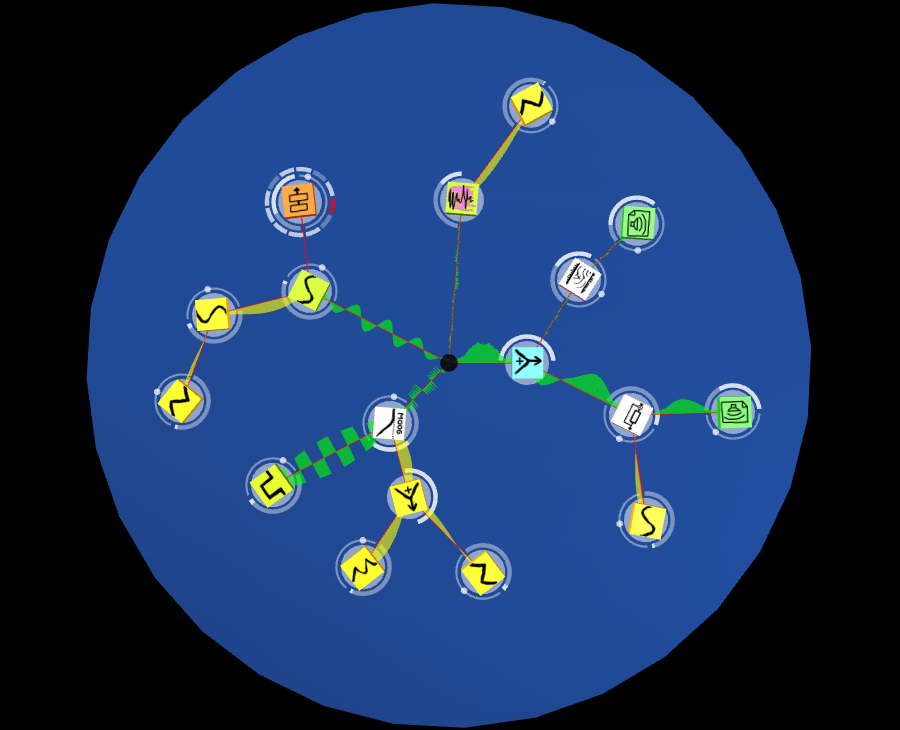
\includegraphics[width=.6\textwidth]{pic/dynamic-patch.png}
\caption{A screenshot of Psychosynth 0.1.1 using dynamic patching to
  connect a complex graph.}
\label{fig:dynamicpatch}
\end{figure}

\subsubsection{Touchable interfaces}

An specific problem for music software is that its interface is highly
limited by the keyboard and mouse as interface. While a person has 20
fingers\footnote{She must be very skilled to use all of them at the
  same time!} she is limited to manipulate only one parameter at a time
with the mouse.

There is an increasing availability of touchable interfaces, either
specifically designed for music performance like the Lemur (figure
\ref{fig:lemur}) or general purpose ones like the IPad. There, one is
no longer constrained by the single-click paradigm and not only can
she manipulate various parameters at a time, different multi-tap
gestures can expand the possibilities of a spatially limited user
interface as several functions can be reached in the same points.

\begin{figure}[h!]
\centering
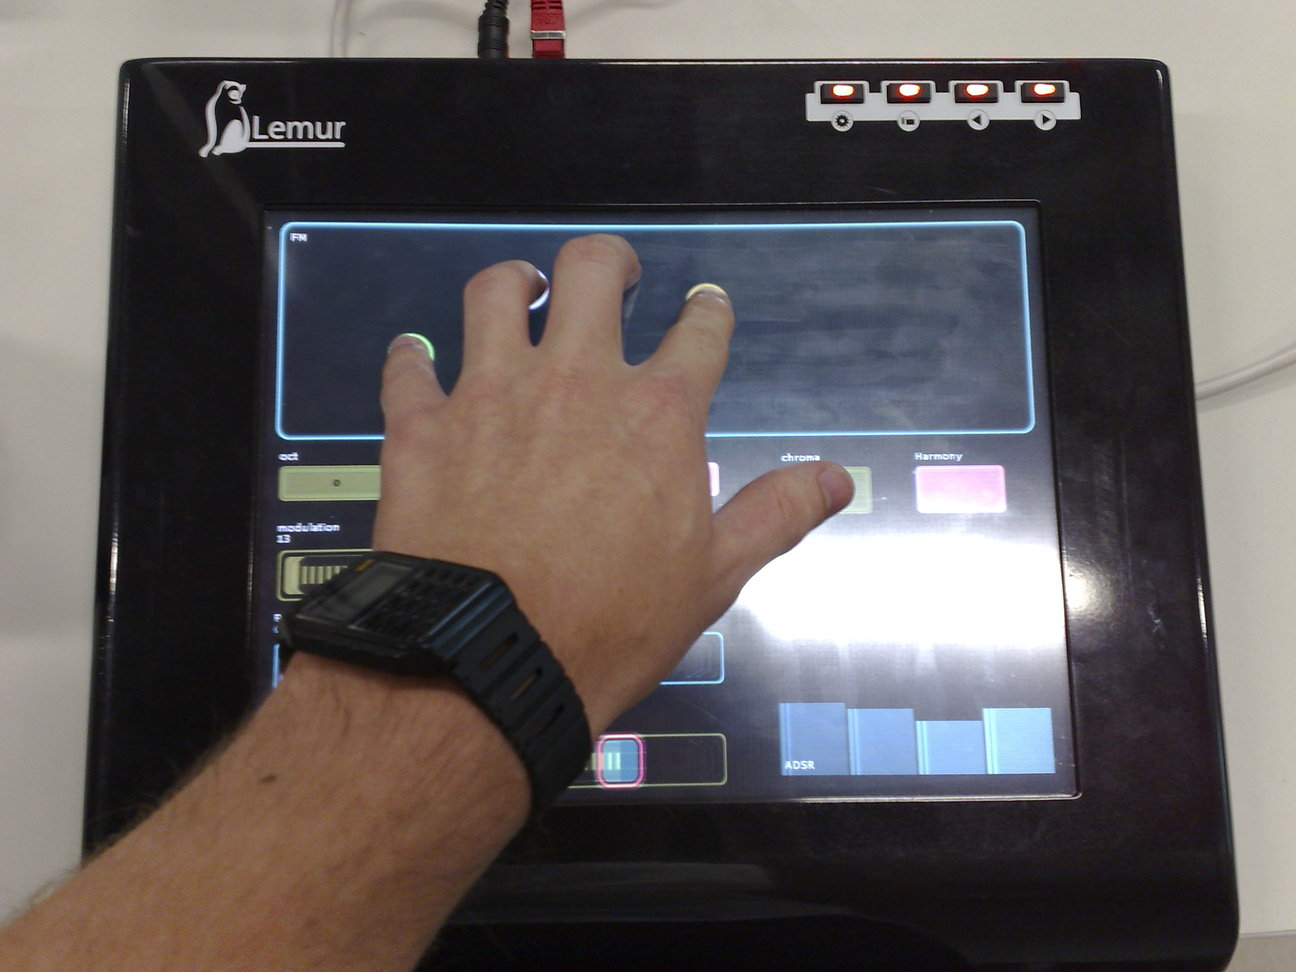
\includegraphics[width=.6\textwidth]{pic/lemur.jpg}
\caption[The JazzMutant's Lemur touchable music interface.]{The
  JazzMutant's Lemur touchable music interface. All the on-screen
  controls can be configured with an UI designer program, and later
  mapped to any program via OSC messages.}
\label{fig:lemur}
\end{figure}

\subsubsection{Instrument simulating controllers}

While touchable interfaces might be better for manipulating the
continuous parameters of the synthesis and dynamically manipulate a
sequencer, many musicians would prefer more traditional interfaces to
interpret part of their work in the ``old-fashioned'' way of playing
an instrument \cite{magnusson07acoustic}. There exists many kinds of
electronic devices that simulate the feel of a keyboard or a drum-kit
(figure \ref{fig:midicontrol}) but instead of producing any sound they
send MIDI \cite{completemidi} messages to a synthesiser that reproduces
the notes.

Our software should be able to interpret MIDI messages such that it
can be controlled with such a device, making it more natural and
creative for many musicians.

\begin{figure}[h!]
\centering
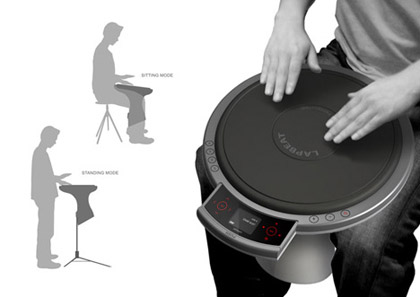
\includegraphics[width=.6\textwidth]{pic/lapbeat.jpg}
\caption[A conga-alike MIDI controller.]{A conga-alike MIDI
  controller. When pressing different parts of its surface it will
  emit different MIDI note messages, that a synthesiser or sampler
  could use to either simulate a real conga or to produce any other
  sound.}
\label{fig:midicontrol}
\end{figure}

\subsection{A collaborative environment}

Since the beginning of times, music performance have been a
collaborative act, with each performer contributing to the global
rhythm and harmony by playing one instrument. Psychosynth should serve
the purpose of producing arbitrarily complex music by itself as
modules that implement not only synthesis, but also sampling and
sequencing are added.

This integrated environment should be able to be manipulated by
several people at the same time to allow a collaborative
experience. After all, it would be very hard for one person to control
in a live performance all the subtleties of the sound generation by
herself.

\subsubsection{Tangible interfaces}

One approach to achieve this is by using a user interface that is big
enough to accommodate several performers around it. A tangible
interface is one where the different elements are represented by
physical objects that one can touch and move in physical space.  The
ReacTable implements such an interface where the modules of its
synthesis engine are plastic blocks that are laid out over a round
table that provides visual feedback thanks to a projector under it. As
shown in figure \ref{fig:reactable}, with such an intuitive and
physically unconstrained interface several people can stand around the
device and manipulate it.

\begin{figure}[h!]
\centering
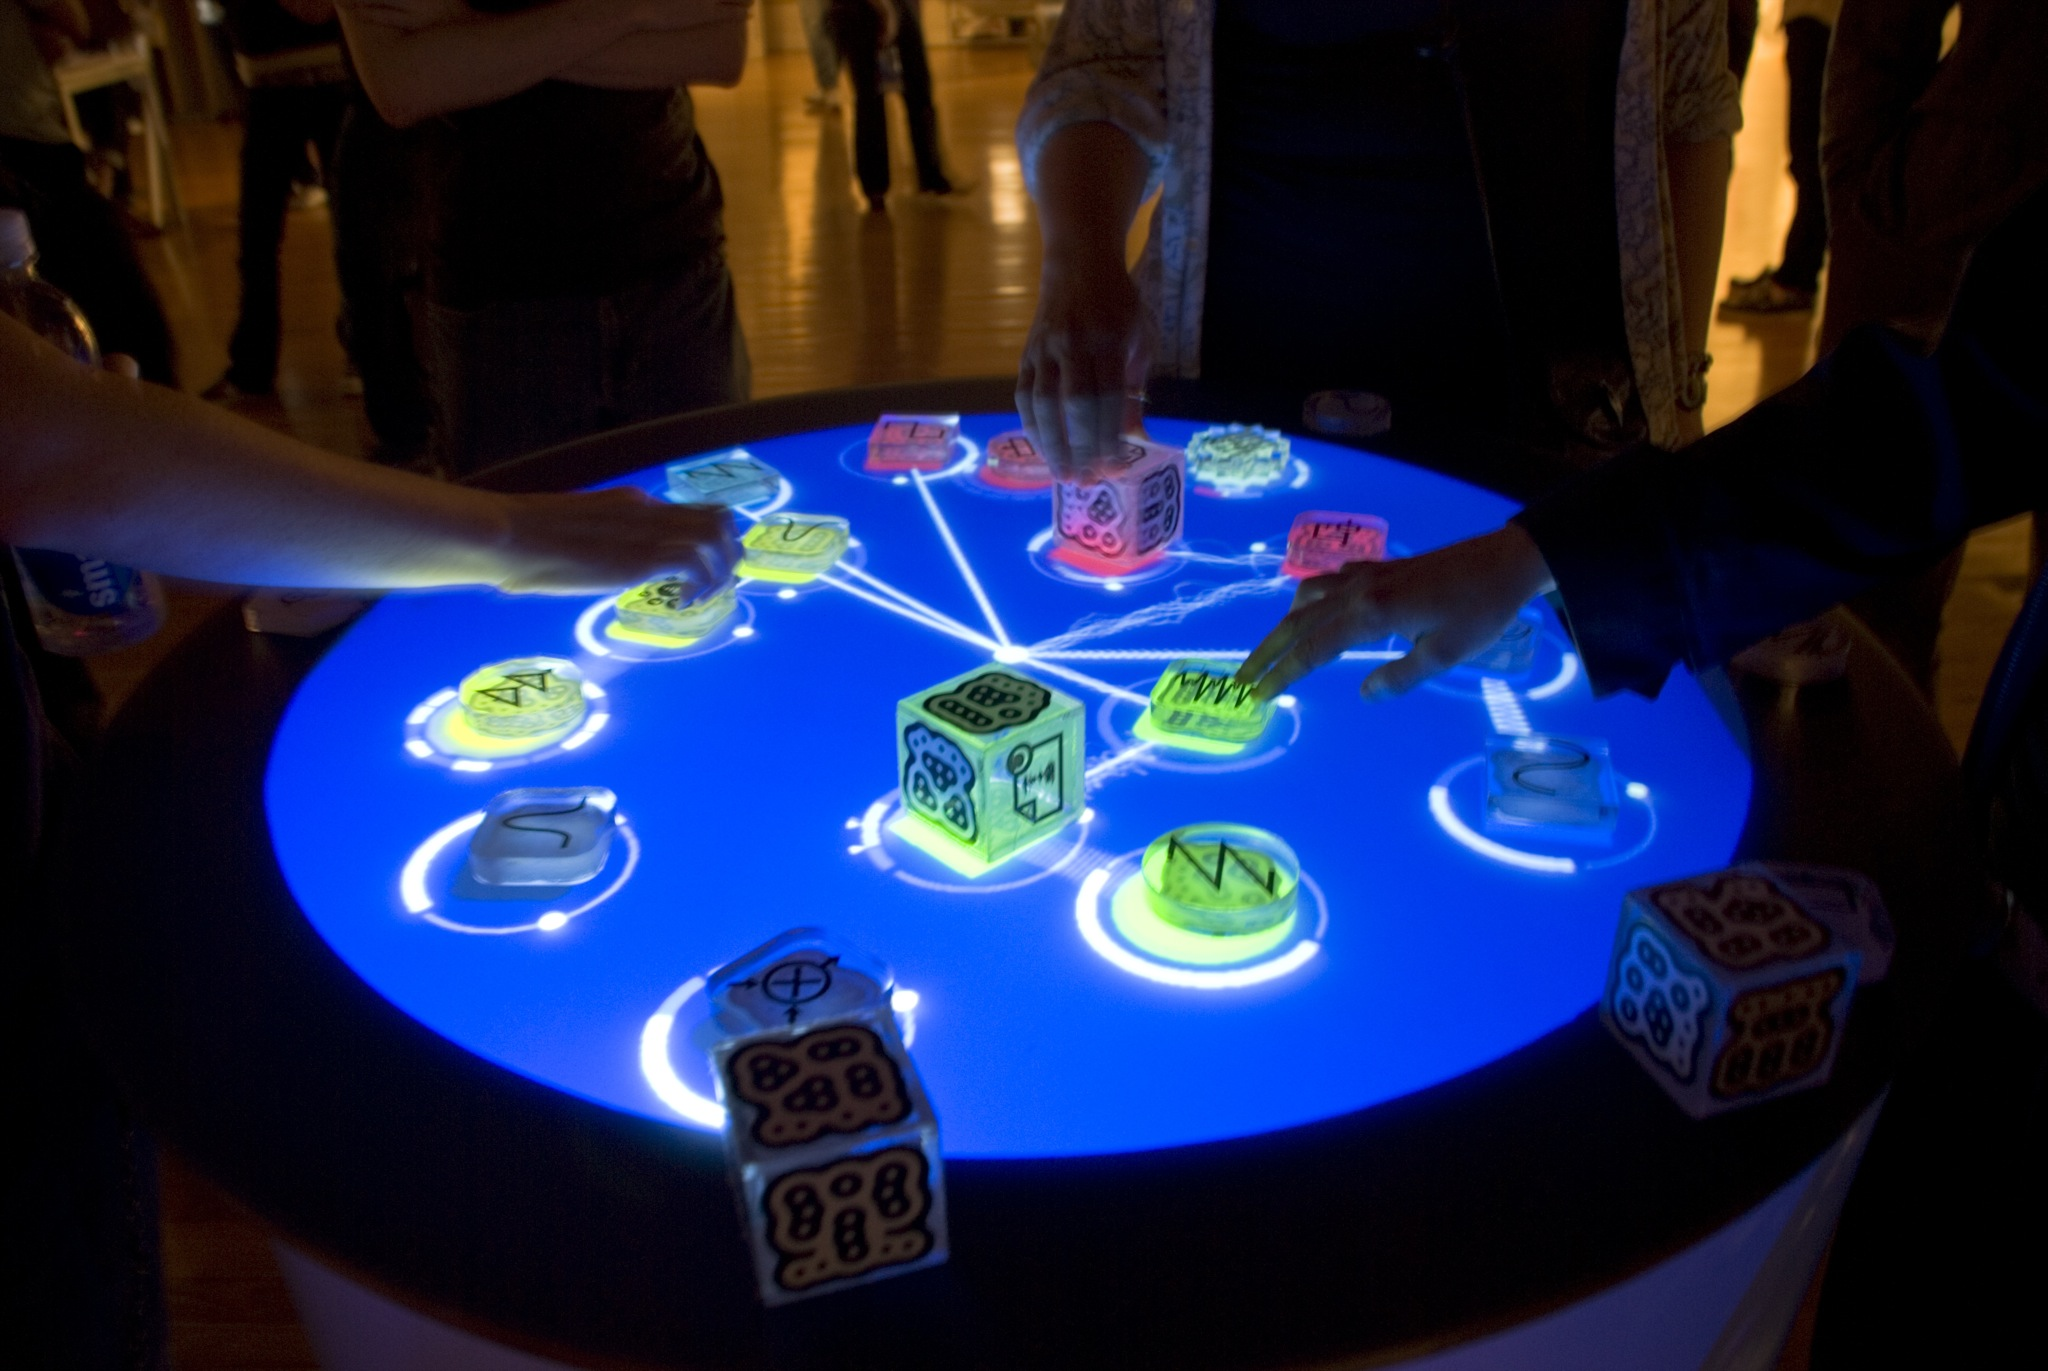
\includegraphics[width=.7\textwidth]{pic/reactable.jpg}
\caption{An example of the Reactable being used collaboratively by
  several people.}
\label{fig:reactable}
\end{figure}

\subsubsection{Networking}

Networking support even further releases a device from the space
constraint by allowing several instances of the software
intercommunicate over a computer network ---i.e. IP. At some point,
latency problems can still be a drawback for this technique, but it
can be useful for some kinds of collaboration that do not require
perfect timing. When playing in a local range, this becomes perfectly
valid even under high latency requirements.

This has long time been a main goal in Psychosynth. When running in
collaborative mode, all the clients that connect to a server share the
same synthesis graph and whenever and object is moved, added or
deleted, or a parameter is changed, all are notified such that they
keep the same view of the scene. Figure \ref{fig:collab} shows an
example of this feature being used live.

\begin{figure}[h!]
\centering
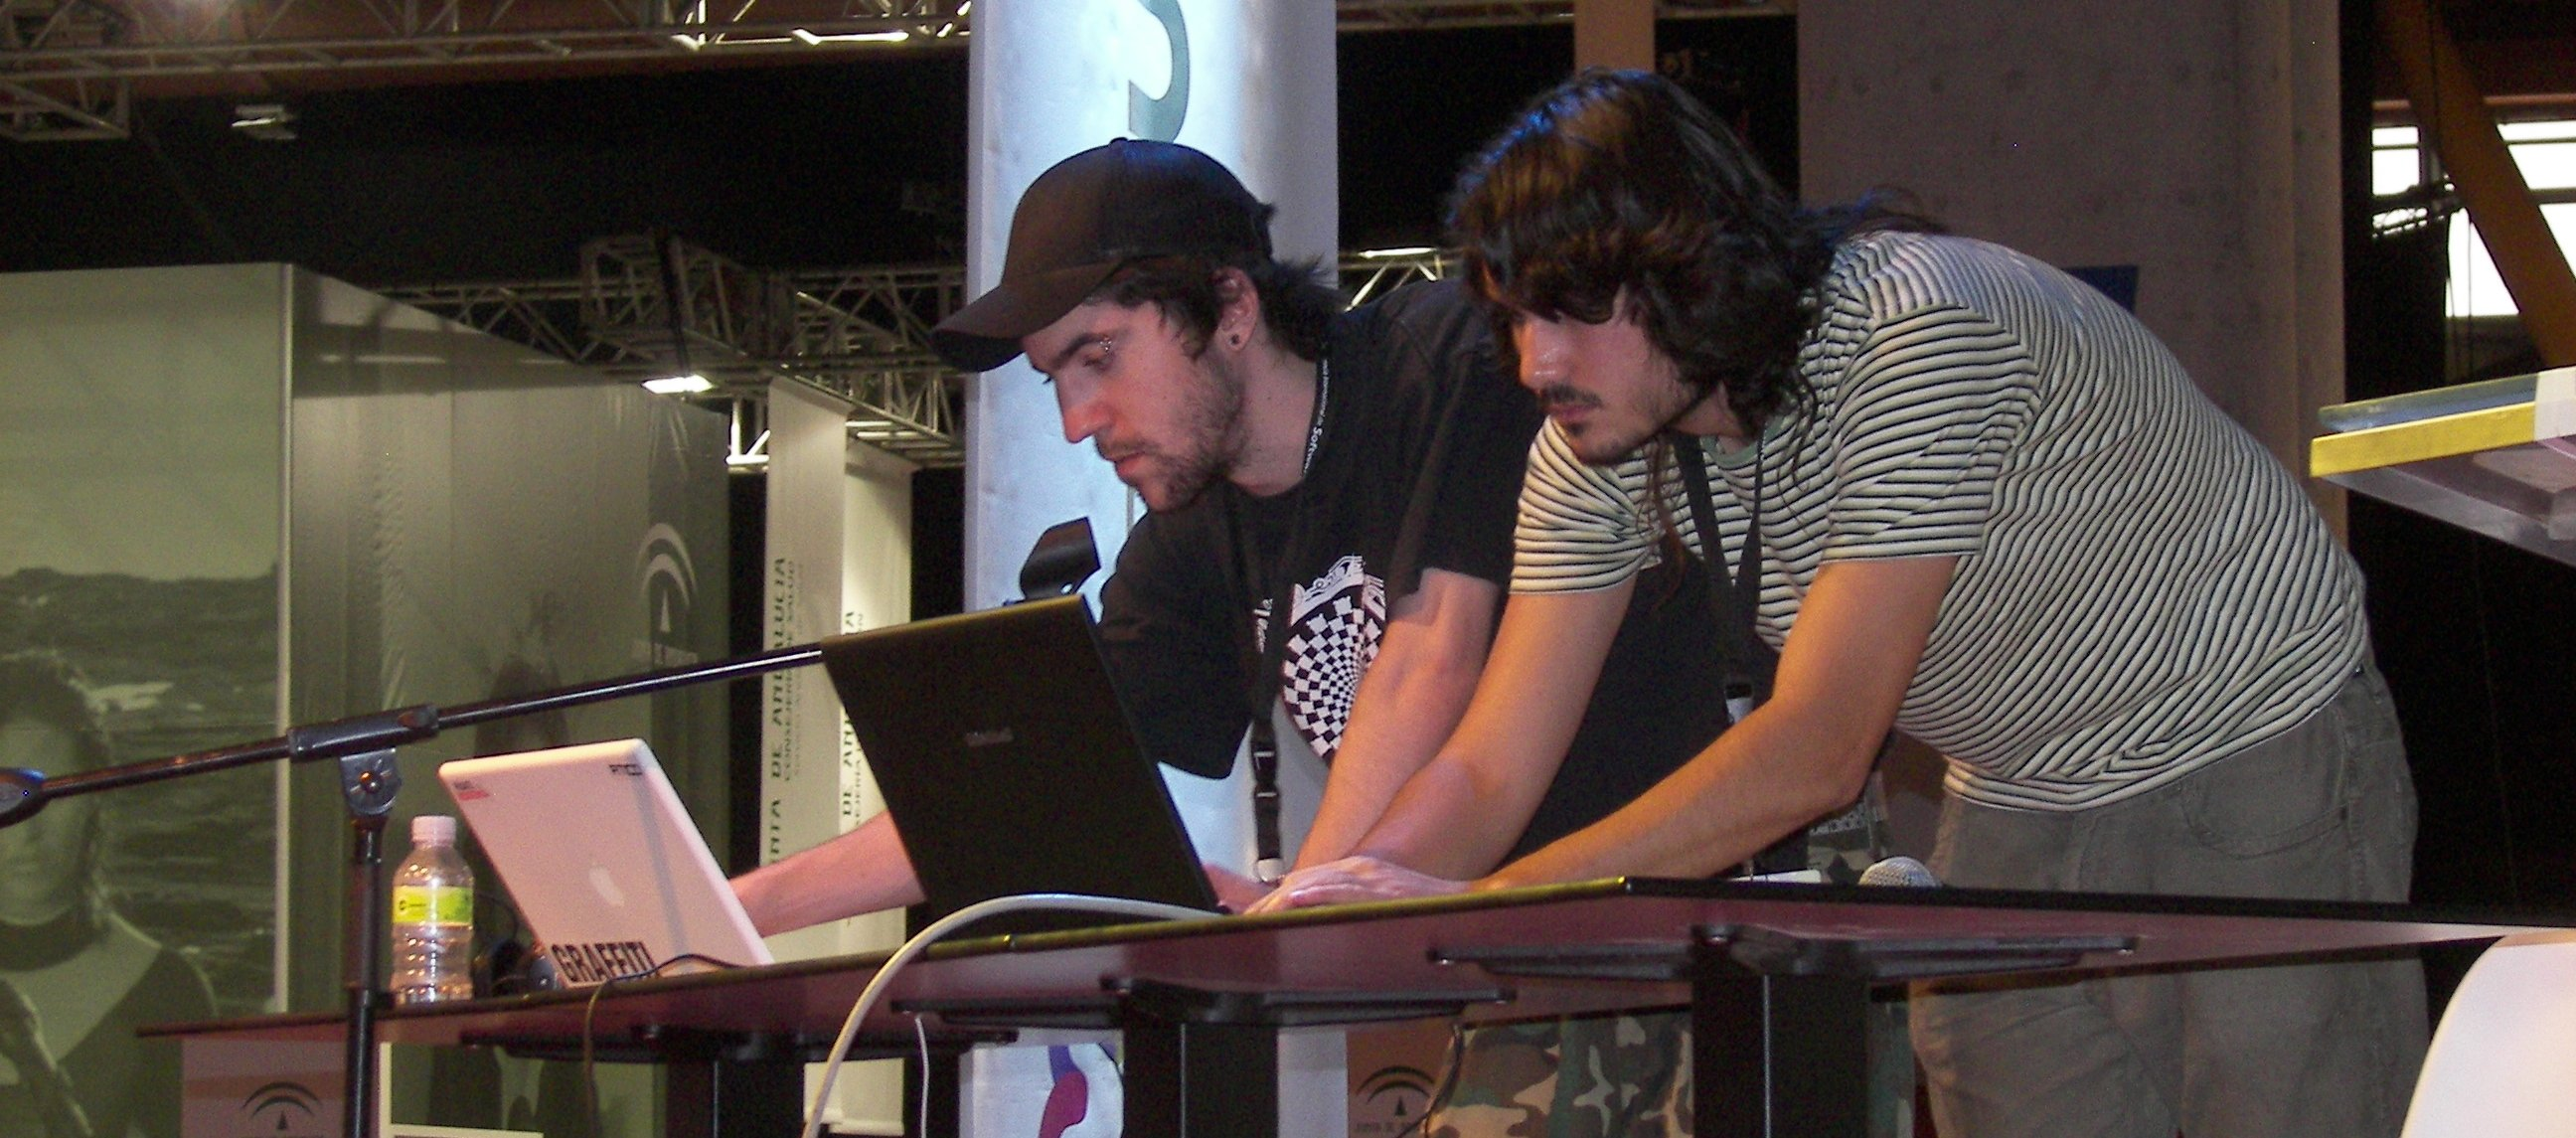
\includegraphics[width=.9\textwidth]{pic/collab.jpg}
\caption[An example of Psychosynth 0.1.4 being used collaboratively
over the network.]{An example of Psychosynth 0.1.4 being used
  collaboratively over the network. The picture was taken in a
  showcase performance held by Shaker08 and the author in the Open
  Source World Conference in 2008.}
\label{fig:collab}
\end{figure}

\subsection{A framework}

Music making and audio processing software and interfaces are evolving
very fast. Abstracting the common core functionality needed by
developers in a layered and abstracted programming API and development
of a Free Software \cite{stallman2002free} framework is crucial to enable
further focused research on the different areas previously
discussed. Results of that research can be later integrated in the
framework as they are stabilised.

Such a framework should enable the development of modular audio
applications with an abstracted interfacing mechanism, probably
following a Model-View-Controller paradigm, general enough to be able
to support all the previously described qualities. If this task is
properly accomplished, the framework could become the basis of a wide
range of unexpected future Free Software applications.

\section{Objectives}

Taking all that into account, we should next define the concrete
objectives for our present project. We should note that we depart from
the basis of the current state of the GNU Psychosynth project ---as of
its version 0.1.7--- and we assume that as previous work, not our
current target.

\subsection{Main objective}
\label{sec:mainobjective}
\label{sec:userinterface}

\begin{objective}
  Re-focus the GNU Psychosynth project as a development framework for
  the development of professional-quality modular, interactive and
  collaborative synthesisers.
\end{objective}

In the long-term we would like GNU Psychosynth to include innovative
user interfaces, and some might even be developed as a side effect of
this project ---or we might just update the older one to rely on the
new framework. However, that is not the purpose of this project,
instead we will concentrate on the development of the underlying core
architecture and implementation of its API.

This is so mainly because of time constraints. Also, if we were to
miss some features in the core in order to allocate more time for the
user interface, we have to take into account that this will probably
hard to fix afterwards when a lot of code depends on the broken
design. Also, user interface development is easier to do in a
non-disciplined, voluntary and heterogeneous team. If we achieve a
nice framework now we can still develop the user interfaces later with
the help of other the people collaborating on the Internet; but, as
these two years of stalled development have shown, it is hard without
the pressure of an external deadline and a project plan to invest a
lot of time in rewriting the ``invisible'' but crucial parts of the
system.

\subsection{Preconditional objectives}

There are two objectives of this project that can also be considered
as a precondition for the success of our main goal. These are:

\begin{objective} \label{obj:artquimia}
Collaborate with professional musicians to get a
defined understanding of the meaning of ``professional quality'' and
their real needs.
\end{objective}

The students participating is this project have an amateur knowledge of
music production. It is important to communicate and allow supervision
by professional musicians and experts in digital music to assure the
suitability of the software for use in a professional environment.

We are working in collaboration with the ArtQuimia Music Production
School\footnote{\url{http://www.artquimia.net/}}, which has long time
been educating successful producers and is currently participating in
the European Cross-Step
project\footnote{\url{http://www.cross-step.org/node/4}}, and his
director David García, a musician with professional experience in the
industry as music composer and sound designer for video games.

\begin{todo}[Juan Pedro]
Me consta que David ha trabajado en la industria de videojuegos
sintetizando sonidos pero debería preguntarle a ver si hay algo más
destacable en su currículum.
\end{todo}

\begin{objective}
  Research and apply the latest techniques in modular design and
  implementation and explore the boundaries of the underlying
  implementation devices.
\end{objective}

The success of an framework relies on the proper decomposition of its
features and its extensibility. Moreover, the authors of this project
have a special fascination for programming languages, design patterns
and software modularity. Even more, there is an active research
community questioning and re-developing the modularisation and
abstraction techniques of the underlying programming language C++,
a fact that is more true as we approach the final resolution of the
standarisation committee on the new C++0x standard. All this suggests
that research and application of the state-of-the-art and even
development of our new design and coding patterns will be one of the
leading objectives during the project and play a leading role in
its overall success.

\subsection{Partial objectives}

A more concrete subdivision of our main goal should be given. Note
that these are not yet the detailed requirements, but an overall
initial objectives vaguely elicited from the problem definition, the
previous experience with the GNU Psychosynth software and our personal
interests.

\begin{objective}
Improve the framework to be able to load modules dynamically from
plug-ins, satisfying our own API and/or third-party standards.
\end{objective}

This is a common feature in most industry standard applications and
ours should support it. Many layers of the framework, specially those
related to the dynamic patching, will require vast modifications to
enable customisation to understand third-party modules.

\begin{objective}
Improve the framework to be able to communicate with music controllers
via MIDI or other industry standards.
\end{objective}

While not explicit in this wording, this adds the requirement for
\emph{polyphony} as in most cases such feature would be useless without
it.

\begin{objective}
Add basic synchronization and sequencing support to the framework.
\end{objective}

If we want to understand the software as a full live performance
environment and not a bare synthesiser, this currently lacking feature
is fundamental.

\begin{objective}
Include common modular audio system utilities into the framework. Some
of the most important being patch hierarchy and persistence. 
\end{objective}


\section{Background and state of the art}

\subsection{Modular synthesis}

The history of modular audio generation starts with the Moog
analog synthesiser in 1967 \cite{moog1964voltage}. Since then, a wide
variety of analog modular synthesisers have been developed
commercially, but retaining some limitations as described in the
introduction in section \ref{sec:defmodular}.

Modular synthesis became more interesting with the uprising of
computer based electronic music. One of the most important examples in
this development is Max/MSP \cite{puckete2002max}. This is a dataflow
based visual programming environment mainly targeted at music
applications. In such software one can add boxes where one types the
name of the function that it should perform. When the name has been
written some connection plugs appear on its corners depending on the
module name, and one can draw lines connecting those plugs. Figure
\ref{fig:autechre} showed an example of its functioning. The author of
Max/MSP later developed a Free Software counterpart called Pure
Data\cite{puckette96puredata} that also has video processing
and synthesis support.

\begin{todo}
  A continuación hablo de aplicaciones comerciales que no tienen (o no
  he encontrado) artículos academicos. Estoy evitando citar los manuales
  de usuario o simplemente enlazar a sus webs comerciales, pero no sé
  que es lo más ortodoxo hacer en estos casos. En algunos casos más
  adelante y cuando lo he considerado relevante estoy poniendo enlaces
  al pie de página cuando no existe un paper académico. Cualquier
  recomendación al respecto es bienvenida.
\end{todo}

Since then, many user-oriented commercial modular synthesisers have
been developed. One of the most famous ones is Native Instrument's
Reaktor (figure \ref{fig:reaktor}). In its version 5 it included the
new \emph{core-cell} technology, which allows the visual and modular
design of the lower level parts of the DSP (Digital Signal
Processing) programming, which transparently compiled to efficient
machine code. Later, Plogue's Bidule is gaining special recognition
for its simpler interface. A new interesting software is XT Software's
EnergyXT, a DAW (Digital Audio Workstation) that has a ``modular
view'' where one can route through wires all the MIDI and audio
signals that flow behind the traditional sequencing view. Finally,
Sensomusic's Usine is remarkable for introducing a highly customisable
multitouch graphical interface on top of a modular synthesis
environment.

\begin{figure}[h!]
\centering
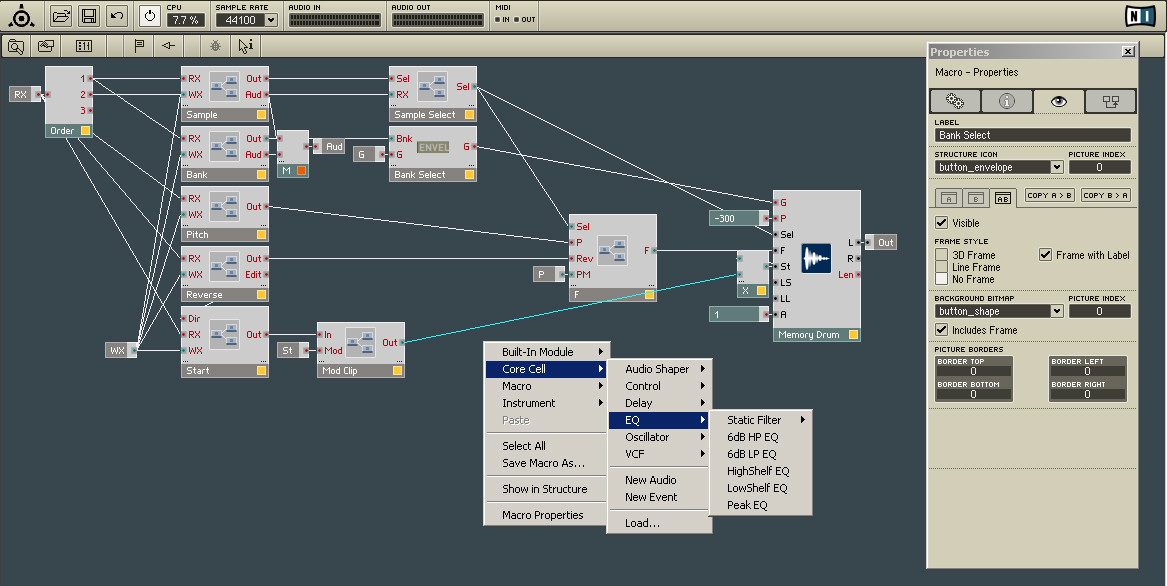
\includegraphics[width=.9\textwidth]{pic/reaktor.jpg}
\caption{Native Instrument's Reaktor editing a \emph{core cell} based
  patch.}
\label{fig:reaktor}
\end{figure}

On the Free Software side few modular synthesisers exist. Alsa Modular
Synth\footnote{\url{http://alsamodular.sourceforge.net/}} is one of
the most
popular. Ingen\footnote{\url{http://drobilla.net/blog/software/ingen/}}
is a more modern one whose code we praise for its quality. Most of
these software still lack some of the features of their privative
counterparts, with the ability to create customised user interfaces
being the most relevant. Still, Free Software offers a very
interesting modular approach to the sound system management that has a
similar rival only in latest OSX versions:
Jack\cite{letz09jack2}. Jack is an audio server providing zero-latency
interprocess communication that acts as a patch-bay among any
supporting audio applications. The user can route the output of one
program to the input of any other program, or the soundcard sink, or
whatever exposes a Jack port. It can be used to route MIDI signals too
and recent versions include very nice features, like collaborative
routing over the network for distributed performances \cite{hohn09netjack}.

\subsection{Touchable and tangible interfaces}

In the last decade, the development of touchable and tangible user
interfaces have been of rising interest. An interesting but not very
updated survey that gives some taxonomical background and analyses a
wide variety of products can be found here
\cite{blaine2003contexts}. One of the first attempts in using them for
improved interaction in musical software is the Audio
Pad\cite{patten2002audiopad}, where the user places and moves tagged
pucks on a bidimensional surface. This is an example of an interface
with active tangibles, because the pucks have an RF transmitter to
allow their recognition. The Jam-o-Drum, on the other hand, offered a
percussive collaborative approach where performers sit on the corner
of an interactive table \cite{blaine00jam}. Many videogames and other
kinds of application have been developed on top of the Jam-o-Drum
hardware too. Since then, a huge number of different table based
interfaces have been made, an example listing can be found
here\footnote{\url{http://mtg.upf.edu/reactable/related.htm}}.

Maybe the most interesting example, which inspired the whole
development of GNU Psychosynth, is the Reactable
project\cite{jorda07thereactable}. Its user interface is based on
modular synthesis and uses the dynamic patching technique for easily
manipulating the patch topology. It uses innovative digital image
processing techniques to detect the position and rotation of passive
tangibles \cite{bencina06improved}. In the Reactable system a
translucid round surface hides a projector and a high resolution
camera underneath, as shown in figure
\ref{fig:reactablesetup}. Finger-tips and the specially designed tags
called \emph{fiducials} that are placed on the table surface are
captured by the camera and recognised by the ReacTIVIsion system on a
computer. This system sends OSC\cite{center03osc} (Open Sound Control) based
messages to a synthesiser following the TUIO (Tangible User Interface
OSC) protocol \cite{kaltenbrunner05tuio}. The literature describing
the initial prototypes used Pure Data as the underlying implementation
language for this synthesis engine, but conversations with the authors
of the Reactable suggest that the current commercial implementation
is written in C++. This synthesis engine is connected to a visual
engine that generates visual feedback and sends it through the
projector. The picture is reversed so it can be correctly visualised
through the translucid surface.

\begin{figure}[h!]
\centering
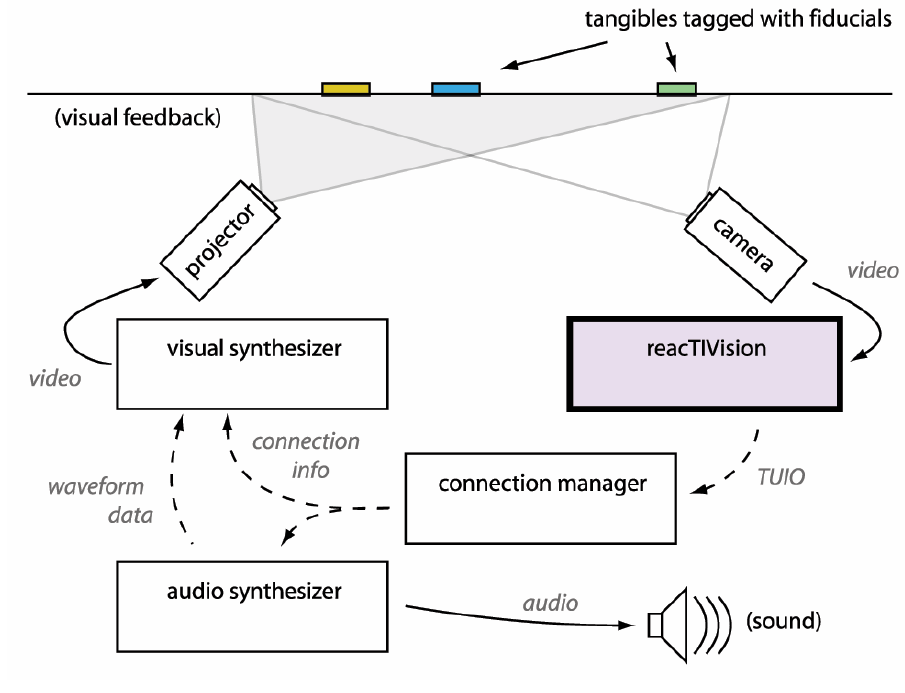
\includegraphics[width=.7\textwidth]{pic/reactable-setup.png}
\caption[A typical Reactable setup.]{A typical Reactable
  setup. Source: The Reactable project.}
\label{fig:reactablesetup}
\end{figure}

The Reactable has been very successful and a very interesting fact is
that the computer vision component of the system is Free Software, so it
could be integrated with GNU Psychosynth in the future.

Some other remarkable tangible and highly interactive user interfaces
that where released around 2007 too are the JazzMutant's Lemur and the
Iwai-Yamaha’s Tenori-On \cite{nishibori06tenorion}. The former offers
a fully customisable OSC based multi-touch interface, where one can
design interfaces with sliders, virtual-knobs, X-Y pads and all kinds
of multi-touch controls that are mapped to OSC messages that can be
interpreted by the audio engine of choice. The later is a 16x16 matrix
of LED illuminated buttons that can be configured in different modes
that provide innovative sequencing mechanisms (figure
\ref{fig:tenorion}).

\begin{figure}[h!]
\centering
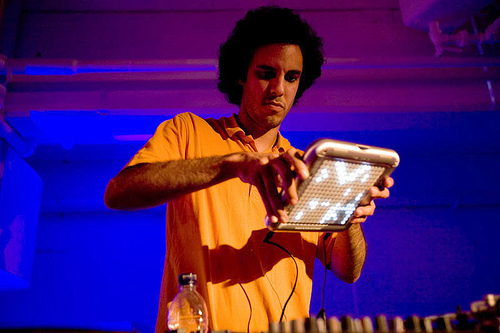
\includegraphics[width=.7\textwidth]{pic/tenorion.jpg}
\caption{Electronic music artist Four Tet performing with a Tenori-On}
\label{fig:tenorion}
\end{figure}

Nowadays, multitouch interfaces are the main trend, specially after
the explosion of the tablet market, but big music software companies
still have to catch up the latest hardware developments. Specially
interesting for the GNU Psychosynth projects it the Indamixxx 2
tablet, which is based on the Meego OS\footnote{Nokia and Intel's
  joint effort to provide a GNU/Linux based operating system for
  embedded devices, mobile phones, netbooks and tablets.} and oriented
towards music production and live performance --- we should definitely
keep an eye on it and develop a multi-touch enabled user interface for
it.

\subsection{Audio synthesis libraries and frameworks}

One of the first synthesis libraries that where evaluated before the
development of GNU Psychosynth started is the STK (Synthesis ToolKit)
\cite{scavone05rtmidi} but it lacks proper dynamic signal routing
mechanisms and some details, like the sample format being hard-coded
to float, seem too constrained.

A popular sound synthesis and music composition DSL (Domain Specific
Language) is CSound, which later was extended with a C and C++
programming API\cite{boulanger00csound}. Many DSP oriented DSLs have
been developed, but they are not general enough to support the
development of the fully featured applications that we wish on top of
GNU Psychosynth. Still, some of them are worth mentioning. Notable
examples are SoundCollider \cite{mccartney2002supercollider}, which
was for a long time the reference sound synthesis DSL; Chuck
\cite{wang03chuck}, that adds concurrency and time control in an
elegant and boilerplate-less fashion, and the newer Faust
\cite{orlarey09faust}, which is based in a functional and data-flow
paradigm and interfaces easily due to its compilation to C++.

While we are focusing on C and C++, many languages have music related
libraries. Impromptu\footnote{\url{http://impromptu.moso.com.au}} is a
Scheme environment for live-coding, this is, live music performances
where the programming is done in front of the audience while the
programmer writes and mutates the code\footnote{The video
  \emph{Algorithms are thoughts, chainsaws are tools}, by Stephen
  Ramsay is a great introduction to this
  technique. \\\url{http://createdigitalmusic.com/2010/07/thought-and-performance-live-coding-music-explained-to-anyone-really/}}. It
supports video manipulation too, but sadly is available for OSX
only. Its heavy modularity and dynamism is what make Lisp dialects so
interesting for live-coding and music composition. Common
Music\cite{taube97common} was started in 1989 and it is a highly
featured Common Lisp framework that, among other things, provides a
very elegant embedded score notation.

Maybe the most similar project to GNU Psychosynth in its approach is
CLAM (C++ Library for Audio and Music) and award winning library based
on modular synthesis\cite{amatriain2006clam}. Its design will be
carefully taken into account during the redesign of few of Psychosynth
core components. Still it does not precisely fit our needs as it is too
oriented toward research simulations and does not support polyphony.

% \begin{todo}
% This is a TO-DO note.
% \end{todo}

%%% Local Variables: 
%%% mode: latex 
%%% TeX-master: "00-main"
%%% End: 
